\documentclass[12pt]{article}

\usepackage{fullpage}
\usepackage{graphicx}
\usepackage{float}
\usepackage[backend=biber]{biblatex}

\title{Untitled}
\author{Pranav Dahiya}
\date{Shiv Nadar University, India\\pd947@snu.edu.in}

\addbibresource{report.bib}

\begin{document}
  \maketitle

  \section*{Abstract}

  A model to predict success or failure of a restaurant can be useful for potential investors. This paper utilized various non-text features extracted from the Yelp dataset and computed relative measures with respect to other restaurants in the vicinity. These features were then used to train a machine learning model to predict the whether or not a given restaurant will shut down in the upcoming year. A new feature, \emph{category\_density} is also introduced. This model gives an accuracy of 71\% on a balanced dataset, improving on the pre-existing state of the art accuracy of 67\%.

  \section{Introduction}

  The restaurant industry has a very high rate of turnover. However, the industry is also volatile, with a significant proportion of restaurants shutting down within a few years of opening. Figure \ref{fig:age} shows the frequency distribution of the age of closed and open restaurants in the dataset. Most restaurants that shutdown, do so within a few years of opening, whereas most restaurants that are open have been so for much longer. A model that can predict whether a given restaurant will remain open or close down after a given period of time will be very important for potential investors. However, this problem is a complex one due to a plethora of factors affecting the result such as location, timing and other economic factors. This project attempts to accomplish this task using business features given in the Yelp dataset \cite{yelp}.

  \begin{figure}[H]
    \centering
    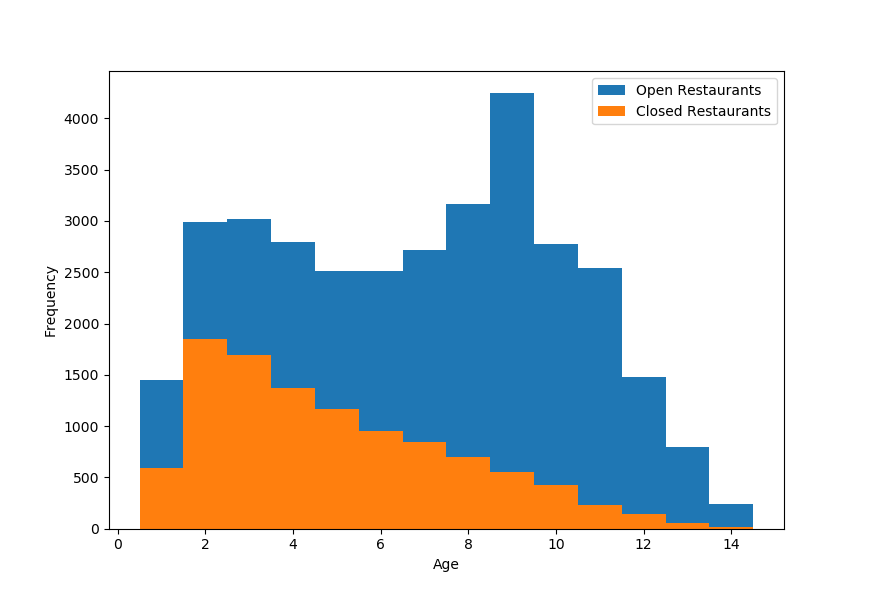
\includegraphics[width=0.7\textwidth]{Figure_1.png}
    \caption{Frequency Distribution of Restaurant Age}
    \label{fig:age}
  \end{figure}

  \section{Related Work}

  Existing work has mostly focused on review data and attempted to use text based features to predict restaurant success or failure. Lu et. al. and Feng et. al. both attempted to incorporate text based features from review data in their classifier and found that they have little to no correlation with the success of a restaurant \cite{Feng16, Lu18}. Therefore, this paper will use only business feature to make a prediction. Alifierakis also attempted to use only business features for classification in \cite{Alifierakis18}. One interesting result from \cite{Alifierakis18} was that the review count feature showed higher correlation with success or failure when it was scaled with respect to the average value of the feature for restaurants in a 1 mile radius. The current state of the art accuracy on a balanced dataset is 67.46\% achieved by Lu et. al. \cite{Lu18}.

  \section{Data Collection}

  Data from the \emph{business, review, tip} and \emph{checkin} files in the Yelp dataset was used to generate the learning set. The first step was to filter out businesses that are not restaurants from the dataset. This was done by selecting entries that have "Restaurant" as one of the business categories. Next, the date of opening and closure of a restaurant had to be determined from the data. While the \emph{business} file contains an \emph{is\_open} attribute, it can only be used to determine whether or not the given restaurant was open or closed when the dataset was released. Therefore, the date of opening and closure for each restaurant was estimated by the date of the first and last review, tip or check-in respectively. Since this date is only an estimate, just the year of opening and closure was noted.\\

  The list of features extracted from the dataset is given in the list below. Features were extracted for each restaurant for each year it was open (except the year of opening and closing). Also, the first check-in for any restaurant in the dataset was in 2010, so only years from 2010 onwards were considered. Finally, the starred features were scaled by the mean value of that feature for restaurants in a 2 km radius that were open in that year.

  \begin{itemize}
    \item \textbf{stars$^*$}: The average star rating in reviews written for the given restaurant in the given year
    \item \textbf{review\_count$^*$}: The total number of reviews written for the given restaurant in the given year
    \item \textbf{tip\_count$^*$}: The total number of tips written for the given restaurant in the given year
    \item \textbf{checkin\_count$^*$}: The total number of check-ins for the given restaurant in the given year
    \item \textbf{age}: Number of years since opening
    \item \textbf{chain}: Natural log of the number of open restaurants with the same name as the given restaurant in the given year
    \item \textbf{density}: The number of open restaurants in a 2 km radius of the given restaurant in the given year
    \item \textbf{category\_density}: The ratio of open restaurants with at least one matching category (excluding "Restaurant" and "Food") to the total number of open restaurants in a 2 km radius of the given restaurant in the given year
    \item \textbf{mean\_stars, mean\_review\_count, mean\_tip\_count, mean\_checkin\_count,\\ mean\_density}: The mean value of the corresponding feature in all years since opening till the given year
  \end{itemize}

  There were a total of 36855 unique restaurants in this dataset, out of which 8065 closed sometime between 2010 and 2017. ML models were trained on this data to attempt a binary classification on whether or not a restaurant will remain open in the upcoming year. So for a restaurant that did shut down, the entry from the year just before the year of shutdown was taken, whereas for restaurants that remained open, the entries from 2017 were considered.\\

  Before training a model on this data, it is first converted to a balanced set and only 8065 open restaurants were randomly chosen from the entire dataset. Then, each feature is scaled by the mean and standard deviation of the feature in the entire learning set. Finally, since there are features in this model that may be highly correlated with each other, PCA was used to decorrelate them.

  \section{Results}

  The correlation coefficient of each of the extracted features with the success of the restaurant is given in table \ref{tab:correlation} below.

  \begin{table}[H]
    \centering
    \caption{Pearson correlation coefficient of features with respect to binary classification output}
    \label{tab:correlation}
    \begin{tabular}{r|l}
      \textbf{Feature Name} & \textbf{Correlation} \\
      \hline
      age & 0.288 \\
      mean\_review\_count & 0.027 \\
      review\_count & 0.057 \\
      chain & 0.289 \\
      mean\_stars & -0.061 \\
      stars & -0.004 \\
      mean\_tip\_count & 0.039 \\
      tip\_count & 0.058 \\
      mean\_checkin\_count & 0.038 \\
      checkin\_count & 0.057 \\
      density & -0.059 \\
      category\_density & 0.117
    \end{tabular}
  \end{table}

  Various metrics for all the classifiers trained on the binary classification problem after 10-fold cross validation are given in table \ref{tab:binary} below.\\

  \begin{table}[H]
    \centering
    \caption{Results of binary classification}
    \label{tab:binary}
    \begin{tabular}{r||c|c|c|c}
      \textbf{Model Name} & \textbf{Accuracy} & \textbf{Precision} & \textbf{F1} & \textbf{Recall}\\
      \hline
      Logistic Regression & 0.68 $\pm$ 0.06 & 0.71 $\pm$ 0.09 & 0.66 $\pm$ 0.04 & 0.63 $\pm$ 0.02 \\
      SVM & 0.69 $\pm$ 0.06 & 0.73 $\pm$ 0.10 & 0.68 $\pm$ 0.05 & 0.65 $\pm$ 0.02 \\
      Neural Network & 0.71 $\pm$ 0.07 & 0.72 $\pm$ 0.09 & 0.71 $\pm$ 0.05 & 0.71 $\pm$ 0.02
    \end{tabular}
  \end{table}

  \section{Discussion}

  Three features that correlate highly with restaurant success are \emph{age, chain} and \emph{category\_density}. This confirms that the right location is essential for restaurant success. Having restaurants serving similar cuisines in the vicinity improves the probability of success. This might be an indicator of the tastes and preferences of consumers in the area. Other review based features, even when adjusted based on the mean value of surrounding restaurants do not correlate very well. This confirms the results of existing research that review based feature (both text and non-text) do not correlate very well with restaurant success. However, just as this research was able to use review data to infer the year of opening and closing for restaurants, this data can be used in other ways. While the tagged attributes of businesses in the dataset other than location and name can be useful for making a prediction regarding its success, not every restaurant is tagged with every attribute. Review data can be used to fill in these gaps. Future work should focus on filling up these gaps using NLP, which may lead to more features that correlate well with restaurant success, thereby including accuracy of predictions. Also, most features were positively correlated with restaurant success. This may imply that while there are some features that can be an indicator of restaurant success, detecting the failure of a restaurant in advance may be a more complicated problem. In conclusion, this research was able to use the relative value of various non-text features to achieve better results on a balanced learning set as compared to pre-existing state of the art.

  \printbibliography

\end{document}
